\documentclass[11pt,oneside]{article}
\usepackage[a4paper,margin=27mm,headheight=15pt]{geometry}
\usepackage[T1]{fontenc}
\usepackage[utf8]{inputenc}
\IfFileExists{libertinus.sty}{\usepackage{libertinus}}{\usepackage{lmodern}}
\usepackage{microtype}
\usepackage{amsmath,amssymb,amsthm,mathtools,mathrsfs}
\usepackage{bm}
\usepackage{booktabs,longtable,array,tabularx}
\usepackage{graphicx}
\usepackage{xcolor}
\usepackage{enumitem}
\usepackage{fancyhdr}
\usepackage{titlesec}
\usepackage{listings}
\usepackage{xurl}
\usepackage{hyperref}
\usepackage[nameinlink,noabbrev]{cleveref}

\definecolor{linkblue}{RGB}{25,75,135}
\definecolor{shadegray}{RGB}{246,247,249}
\definecolor{rulegray}{RGB}{195,201,208}
\definecolor{provedgreen}{RGB}{25,105,70}
\definecolor{conjecturered}{RGB}{150,45,45}
\hypersetup{
  colorlinks=true,
  linkcolor=linkblue,
  citecolor=linkblue,
  urlcolor=linkblue,
  pdftitle={Beyond the Dyadic Fabius Web},
  pdfsubject={A geometric q-Fabius--Rvachev family, endpoint laws, zero arithmetic, and phase-aware extrapolation},
  pdfkeywords={Fabius function, inverse Fabius function, Rvachev up-function, Thue-Morse, q-binomial, sinc product, Lambert W, Bell polynomial, Bernoulli polynomial, Richardson extrapolation}
}

\pagestyle{fancy}
\fancyhf{}
\fancyhead[L]{\small Beyond the dyadic Fabius web}
\fancyhead[R]{\small\nouppercase{\leftmark}}
\fancyfoot[C]{\thepage}
\renewcommand{\headrulewidth}{0.4pt}
\titleformat{\section}{\Large\bfseries}{\thesection}{0.7em}{}
\titleformat{\subsection}{\large\bfseries}{\thesubsection}{0.7em}{}
\titleformat{\subsubsection}{\normalsize\bfseries}{\thesubsubsection}{0.7em}{}
\setcounter{secnumdepth}{3}
\setcounter{tocdepth}{2}
\setlist[itemize]{leftmargin=2em,itemsep=0.25em,topsep=0.4em}
\setlist[enumerate]{leftmargin=2.3em,itemsep=0.25em,topsep=0.4em}
\setlength{\emergencystretch}{2em}

\newtheorem{theorem}{Theorem}[section]
\newtheorem{proposition}[theorem]{Proposition}
\newtheorem{lemma}[theorem]{Lemma}
\newtheorem{corollary}[theorem]{Corollary}
\newtheorem{conjecture}[theorem]{Conjecture}
\newtheorem{problem}[theorem]{Problem}
\theoremstyle{definition}
\newtheorem{definition}[theorem]{Definition}
\newtheorem{algorithm}[theorem]{Algorithm}
\newtheorem{example}[theorem]{Example}
\theoremstyle{remark}
\newtheorem{remark}[theorem]{Remark}
\newtheorem{warning}[theorem]{Warning}

\newcommand{\R}{\mathbb R}
\newcommand{\C}{\mathbb C}
\newcommand{\Q}{\mathbb Q}
\newcommand{\N}{\mathbb N}
\newcommand{\Z}{\mathbb Z}
\newcommand{\E}{\mathbb E}
\newcommand{\Prob}{\mathbb P}
\newcommand{\Var}{\operatorname{Var}}
\newcommand{\Cov}{\operatorname{Cov}}
\newcommand{\supp}{\operatorname{supp}}
\newcommand{\sinc}{\operatorname{sinc}}
\newcommand{\e}{\mathrm e}
\newcommand{\ii}{\mathrm i}
\newcommand{\dd}{\,\mathrm d}
\newcommand{\bigO}{\mathcal O}
\newcommand{\smallo}{o}
\newcommand{\Up}{\operatorname{up}}
\newcommand{\wt}{\operatorname{wt}_2}
\newcommand{\qbinom}[3]{\genfrac{[}{]}{0pt}{}{#1}{#2}_{#3}}
\newcommand{\Law}{\mathcal L}
\newcommand{\Normal}{\mathcal N}
\newcommand{\He}{\operatorname{He}}
\newcommand{\diag}{\operatorname{diag}}
\newcommand{\convexorder}{\preceq_{\mathrm{cx}}}

\newenvironment{boxedremark}{%
  \par\smallskip\noindent\begin{center}\begin{minipage}{0.94\textwidth}%
  \color{black}\hrule\vspace{0.6em}\small
}{%
  \vspace{0.6em}\hrule\end{minipage}\end{center}\smallskip
}

\lstdefinestyle{code}{
  basicstyle=\ttfamily\small,
  backgroundcolor=\color{shadegray},
  frame=single,
  rulecolor=\color{rulegray},
  columns=fullflexible,
  keepspaces=true,
  showstringspaces=false,
  breaklines=true,
  xleftmargin=0.7em,
  xrightmargin=0.7em,
  aboveskip=0.8em,
  belowskip=0.8em
}

\title{\bfseries Beyond the Dyadic Fabius Web\\[0.35em]
\large A geometric $q$-Fabius--Rvachev family, endpoint laws, zero arithmetic,\\
Bernoulli--Bell polynomial calculus, and phase-aware extrapolation}
\author{\small Frontier research report based on the complete \texttt{ProveIt}\\Fabius documentation corpus}
\date{Repository snapshot: 27 August 2026\\
\small \texttt{24da985eba70e46d862acdaddd476793a428213e}}

\begin{document}
\maketitle

\begin{abstract}
The dyadic Fabius function, its inverse, Rvachev's compactly supported up-function,
and the signed Thue--Morse extension form an unusually dense network of exact identities.
The inspected repository already develops that network at considerable depth: exact dyadic
values, Gaussian-binomial coefficient extraction, Bernoulli and Bell polynomial formulas,
Lambert-$W$ endpoint phases, geometric Lagrange interpolation, Richardson filters, and an
extensive campaign on the decay of the infinite sinc product.  This report therefore does
not attempt another rearrangement of those results.  Instead it moves in a transverse
direction by replacing the dyadic ratio $1/2$ by a free geometric parameter $0<q<1$.

For independent $U_j\sim\mathrm{Unif}(0,1)$, define
\[
 X_q=(1-q)\sum_{j\ge0}q^jU_j,
 \qquad F_q(x)=\Prob(X_q\le x),
 \qquad Y_q=2X_q-1.
\]
At $q=1/2$ this is exactly the bounded Fabius distribution, and the density of $Y_{1/2}$
is Rvachev's up-function.  For the full family we prove a refinement equation and a
rapidly decaying infinite sinc product; exact Bernoulli cumulants and Bell moments; a
Bernoulli--Appell polynomial inverse to geometric uniform averaging; a finite-stage
$q$-binomial scale identity; monotone contraction in convex order; an exact shape phase
transition with a central plateau precisely when $q<1/2$; a Gaussian degeneration as
$q\uparrow1$ with explicit standardized cumulants; a two-term logarithmic endpoint law
\[
 \log F_q(x)
 =-\frac{\log^2(1/x)}{2\log(1/q)}
  -\frac{\log(1/x)\log\log(1/x)}{\log(1/q)}
  +\bigO_q(\log(1/x));
\]
and its inverse Lambert-$W$ quantile law.  We also determine Fourier-zero multiplicities
for reciprocal-integer ratios, isolate the arithmetic condition for cross-scale collisions,
and explain why base two alone converts the finite product into a contiguous Thue--Morse
block.  Finally, we give a phase-preserving Lagrange/Richardson filter for asymptotic
remainders whose coefficients are periodic in a lower-Lambert phase, together with a
Fourier phase-averaging filter and exact Lambert-$W$ node construction.

The word \emph{new} is used only in a corpus-relative sense: these statements were not found
in the 57 TeX sources inspected in the specified repository snapshot.  No claim of global
priority is made.  Proven statements are separated sharply from conjectural transseries,
strict log-concavity, Edgeworth, inverse-phase, and arithmetic-collision problems.
Deterministic numerical experiments and all plotting code accompany the report.
\end{abstract}

\begin{boxedremark}
\textbf{Status convention.}
A theorem or proposition in this report is accompanied by an argument intended to be
mathematically complete at the paper level.  A conjecture is explicitly labeled and is not
asserted as proved.  None of the new statements has been formalized in Lean as part of the
repository snapshot.  The principal novelty filter was comparison against all 57 TeX files
listed in \texttt{corpus\_inventory.txt}, including frozen versions, the living syntheses,
the Thue--Morse atlas, all included paper sources, and the twelve Fourier-decay drafts and
audits.
\end{boxedremark}

\tableofcontents
\newpage

\section{Corpus audit and the novelty boundary}
\label{sec:corpus}

\subsection{What was inspected}

The requested tree contains four logically different kinds of material.
First are the living synthesis documents: the primary Fabius--Rvachev exposition, the
mathematical glossary, the Lean walkthrough, the non-elementarity article, the consolidated
frontier volume, and the living Thue--Morse formula atlas.  Second is a twelve-document
Fourier-decay campaign containing proposed analyses, final syntheses, a gentle guide, and two
comparative audits.  Third is a seven-source paper library, including both the original and
corrected TeX of one OCR conversion.  Fourth is a frozen archive of thirty-two historical
versions organized by provenance and topic.  The resulting count is
\[
 6+12+7+32=57.
\]
The exact paths are reproduced in \Cref{app:inventory} and in the companion plain-text
ledger.  The repository's own archive README states that byte-identical historical copies
were pruned and that the archive is grouped by purpose rather than serving as a naive mirror
of every earlier path \cite{proveitArchive}.  Thus the historical sources were treated as a
novelty/provenance map, while the current synthesis documents were treated as the canonical
statement of what the project already contains.

\subsection{What the repository already does very well}

The current primary exposition and frontier synthesis already cover, among much else,
\begin{itemize}
\item the probabilistic construction of the Fabius distribution and the Rvachev bump;
\item exact dyadic evaluation, recurrences, bit-recursive algorithms, and denominator
      arithmetic;
\item Gaussian-binomial and $q$-Pochhammer structures at the fixed base $q=1/2$;
\item Bernoulli cumulants, Bell-polynomial moments, Appell-type blocks, and exact coefficient
      extraction;
\item geometric-node Lagrange identities and $q$-Richardson cancellation of geometric error
      modes;
\item lower-Lambert endpoint variables, nonconstant periodic correction functions, and
      all-orders saddle machinery;
\item the inverse Fabius function, totalization conventions, and dyadic inverse formulas;
\item repeated-integration and box-spline approximants;
\item extensive Thue--Morse identities, rarefied sums, Mahler equations, natural-boundary
      phenomena, and quantitative approximation questions;
\item the quadratic logarithmic envelope, exceptional zeros, and several amplitude notions
      for the Fourier image of the up-function.
\end{itemize}
These features are visible in the primary exposition \cite{proveitPrimary}, the consolidated
frontier volume \cite{proveitFrontiers}, the living atlas \cite{proveitAtlas}, and the
Fourier audit campaign \cite{proveitFourierAudit}.  The fixed-base $q$-calculus is especially
important for the present report: the archive explicitly describes those documents as
\emph{base-$1/2$} articles \cite{proveitArchive}.  Likewise, the archive records an existing
``phase locking'' mechanism for dyadic coefficient extraction.  Accordingly, neither
Gaussian-binomial notation nor phase locking by itself is claimed as new below.

\subsection{Deliberate exclusions}

Three tempting projects were rejected because they would duplicate the corpus too closely.

\begin{enumerate}
\item We do not offer a thirteenth derivation of the leading Fourier decay
\(
 \log|\widehat\Up(t)|\asymp-(\log|t|)^2/(2\log2)
\)
with the known zero-set and limsup qualifications.  The live Fourier drafts compare precisely
such arguments.
\item We do not repackage the exact dyadic value web, the half-base Gaussian-binomial
interpolation formula, or the existing geometric Richardson filter.
\item We do not relabel the existing dyadic lower-Lambert periodic asymptotic as a new
``transseries.''  The new phase-aware extrapolation theorem in \Cref{sec:phase} applies to a
different numerical geometry: inverse powers of a Lambert variable while its fractional
phase is held fixed.
\end{enumerate}

\subsection{The transverse direction}

The central observation is that the dyadic distribution is one member of a natural geometric
one-parameter family.  Making the ratio variable simultaneously exposes:
\begin{itemize}
\item a shape transition at the dyadic value $q=1/2$;
\item a majorization order in the parameter;
\item a Gaussian limit as the geometric mesh becomes diffuse;
\item a general Bernoulli--Bell calculus whose dyadic specialization recovers the repository's
      formulas exactly;
\item a change in Fourier-zero arithmetic from generic simple zeros to valuation-controlled
      multiplicities;
\item a precise reason that the Thue--Morse block is special to base two.
\end{itemize}
This parameter deformation is the organizing principle of the report.

\section{The geometric \texorpdfstring{$q$}{q}-Fabius--Rvachev family}
\label{sec:family}

Throughout, fix
\[
 0<q<1,
 \qquad c=1-q,
 \qquad a=\log(1/q)>0.
\]
Let $(U_j)_{j\ge0}$ be independent random variables, each uniform on $[0,1]$.

\begin{definition}[Geometric Fabius law]
\label{def:qfabius}
Define
\begin{equation}
 X_q=c\sum_{j=0}^{\infty}q^jU_j,
 \qquad
 Z_q=X_q-\frac12,
 \qquad
 Y_q=2Z_q=2X_q-1.                         \label{eq:q-law}
\end{equation}
Write $F_q$ for the extended cumulative distribution function of $X_q$,
$f_q$ for its density, and $u_q$ for the density of $Y_q$.
\end{definition}

Because $0\le U_j\le1$ and $c\sum q^j=1$, the series converges absolutely almost surely and
$X_q\in[0,1]$.  Replacing every $U_j$ by $1-U_j$ shows
\begin{equation}
 X_q\overset d=1-X_q,
 \qquad F_q(x)=1-F_q(1-x),
 \qquad f_q(x)=f_q(1-x).                   \label{eq:symmetry}
\end{equation}
The support is all of $[0,1]$: every open subinterval of $[0,1]$ receives positive
probability by constraining finitely many $U_j$ and leaving a sufficiently short tail free.

\subsection{Recovery of the classical functions}

At $q=1/2$,
\[
 X_{1/2}=\sum_{j\ge0}2^{-j-1}U_j.
\]
This is the standard bounded Fabius distribution.  Moreover, if
$V_j=2U_j-1\sim\mathrm{Unif}[-1,1]$, then
\[
 Y_{1/2}=\sum_{j\ge0}2^{-j-1}V_j,
 \qquad
 \widehat u_{1/2}(t)=\prod_{j\ge1}\sinc(t/2^j),
\]
which is Rvachev's normalized up-function.  The affine relation between densities is
\begin{equation}
 u_q(y)=\frac12 f_q\!\left(\frac{y+1}{2}\right),
 \qquad
 f_q(x)=2u_q(2x-1).                         \label{eq:affine-density}
\end{equation}
Thus the free parameter deforms the Fabius CDF and the Rvachev bump simultaneously.

\subsection{Distributional refinement}

Let $X_q'$ be an independent copy of $X_q$.  Splitting off the first summand gives the basic
self-similarity.

\begin{proposition}[Affine refinement law]
\label{prop:refinement}
One has
\begin{equation}
 X_q\overset d=cU_0+qX_q'.                  \label{eq:distributional-refinement}
\end{equation}
With the convention $F_q(x)=0$ for $x\le0$ and $F_q(x)=1$ for $x\ge1$,
\begin{align}
 F_q(x)
 &=\int_0^1 F_q\!\left(\frac{x-cu}{q}\right)\dd u            \label{eq:cdf-refinement-a}\\
 &=\frac{q}{c}\int_{(x-c)/q}^{x/q}F_q(v)\dd v,               \label{eq:cdf-refinement-b}\\
 f_q(x)
 &=\frac{F_q(x/q)-F_q((x-c)/q)}{c}.                            \label{eq:density-refinement}
\end{align}
\end{proposition}

\begin{proof}
Equation \eqref{eq:distributional-refinement} is the index shift
\[
 c\sum_{j\ge0}q^jU_j=cU_0+q\left(c\sum_{j\ge0}q^jU_{j+1}\right).
\]
Conditioning on $U_0$ gives \eqref{eq:cdf-refinement-a}.  The substitution
$v=(x-cu)/q$ yields \eqref{eq:cdf-refinement-b}, and differentiation gives
\eqref{eq:density-refinement}; smoothness needed for the differentiation follows from
\Cref{thm:smoothness} below, or one may first interpret the derivative distributionally.
\end{proof}

For $q=1/2$ and $0\le x\le1/2$, the second term in
\eqref{eq:density-refinement} vanishes, so
\[
 f_{1/2}(x)=2F_{1/2}(2x),
\]
the classical Fabius differential equation in bounded-CDF normalization.

Repeated differentiation gives a useful hierarchy.

\begin{corollary}[Derivative refinement]
\label{cor:derivative-refinement}
For every integer $r\ge1$,
\begin{equation}
 f_q^{(r)}(x)
 =\frac{f_q^{(r-1)}(x/q)-f_q^{(r-1)}((x-c)/q)}{c q^r}.         \label{eq:derivative-refinement}
\end{equation}
In particular, every derivative vanishes at both endpoints of the support.
\end{corollary}

\section{Infinite sinc products and smooth compact support}
\label{sec:fourier}

The centered uniform variable $U-1/2$ has characteristic function
$\sinc(t/2)$.  Independence therefore gives an infinite product.

\begin{theorem}[Fourier product and rapid polynomial decay]
\label{thm:smoothness}
The characteristic functions of $Z_q$ and $Y_q$ are
\begin{align}
 \phi_q(t):=\E\e^{\ii tZ_q}
 &=\prod_{j=0}^{\infty}\sinc\!\left(\frac{cq^jt}{2}\right),  \label{eq:phi-z}\\
 \widehat u_q(t)=\E\e^{\ii tY_q}
 &=\prod_{j=0}^{\infty}\sinc(cq^jt).                         \label{eq:phi-y}
\end{align}
For every integer $N\ge1$ and every $t\ne0$,
\begin{equation}
 |\phi_q(t)|
 \le \left(\frac{2}{c}\right)^N q^{-N(N-1)/2}|t|^{-N}.      \label{eq:rapid-bound}
\end{equation}
Consequently $X_q$ and $Y_q$ possess compactly supported $C^\infty$ densities, and all
of their derivatives are obtained by absolutely convergent Fourier inversion.
\end{theorem}

\begin{proof}
The product formulas follow from independence and the identity
\(
 \E\e^{\ii s(U-1/2)}=\sinc(s/2).
\)
The product converges locally uniformly because
$1-\sinc z=\bigO(z^2)$ and $\sum q^{2j}<\infty$.
For the first $N$ factors, use $|\sinc x|\le\min(1,|x|^{-1})$; bound all remaining factors by
one.  This gives
\[
 |\phi_q(t)|
 \le\prod_{j=0}^{N-1}\frac{2}{cq^j|t|}
 =\left(\frac{2}{c}\right)^Nq^{-N(N-1)/2}|t|^{-N}.
\]
Given $r\ge0$, choose $N>r+1$.  Then $t^r\phi_q(t)\in L^1(\R)$, so Fourier inversion gives a
continuous $r$th derivative.  Since $r$ is arbitrary, the density is $C^\infty$.  Compact
support was already established from the random series.
\end{proof}

\begin{remark}[Relation to the existing Fourier-decay campaign]
Bound \eqref{eq:rapid-bound} is intentionally elementary.  Optimizing $N$ as a function of
$|t|$ recovers a quadratic logarithmic envelope, but the dyadic case has already been
analyzed in much finer arithmetic and phase detail in the repository.  The genuinely new
content here is the $q$-deformation and the zero arithmetic in \Cref{sec:zeros}, not a claim
of a new sharp dyadic envelope.
\end{remark}

\section{Bernoulli cumulants, Bell moments, and \texorpdfstring{$q$}{q}-binomial scale geometry}
\label{sec:bell}

\subsection{Exact cumulants}

Let $B_n$ denote the Bernoulli numbers in the convention
\[
 \frac{t}{\e^t-1}=\sum_{n\ge0}B_n\frac{t^n}{n!},
 \qquad B_1=-\frac12.
\]
For a uniform random variable $U$ on $[0,1]$, the cumulants are
$\kappa_1(U)=1/2$ and $\kappa_n(U)=B_n/n$ for $n\ge2$.

\begin{theorem}[Bernoulli cumulants]
\label{thm:cumulants}
For the centered law $Z_q=X_q-1/2$,
\begin{equation}
 \kappa_{2m+1}(Z_q)=0\quad(m\ge0),                            \label{eq:odd-cumulants}
\end{equation}
where the case $m=0$ means $\kappa_1=0$, and
\begin{equation}
 \boxed{\displaystyle
 \kappa_{2m}(Z_q)
 =\frac{B_{2m}}{2m}\frac{(1-q)^{2m}}{1-q^{2m}}}
 \qquad(m\ge1).                                             \label{eq:q-cumulants}
\end{equation}
In particular,
\begin{equation}
 \sigma_q^2:=\Var(X_q)=\frac{1-q}{12(1+q)}.                  \label{eq:variance}
\end{equation}
At $q=1/2$,
\begin{equation}
 \kappa_{2m}(Z_{1/2})
 =\frac{B_{2m}}{2m(2^{2m}-1)},                               \label{eq:dyadic-cumulants}
\end{equation}
exactly the dyadic Bernoulli-cumulant formula already present in the repository.
\end{theorem}

\begin{proof}
Cumulants add over independent sums and scale homogeneously.  Hence for $n\ge2$,
\[
 \kappa_n(Z_q)
 =\sum_{j\ge0}(cq^j)^n\kappa_n(U_j-1/2)
 =\frac{B_n}{n}\frac{c^n}{1-q^n}.
\]
All odd Bernoulli numbers beyond $B_1$ vanish, while symmetry gives the vanishing first
cumulant.  Substituting $n=2$ yields \eqref{eq:variance}; substituting $q=1/2$ gives
\eqref{eq:dyadic-cumulants}.
\end{proof}

\subsection{Bell-polynomial moments and a triangular recurrence}

Let $\mathcal B_n(x_1,\ldots,x_n)$ denote the complete exponential Bell polynomial,
characterized by
\[
 \exp\left(\sum_{r\ge1}x_r\frac{t^r}{r!}\right)
 =\sum_{n\ge0}\mathcal B_n(x_1,\ldots,x_n)\frac{t^n}{n!}.
\]

\begin{corollary}[Exact moments]
\label{cor:bell-moments}
For every $n\ge0$,
\begin{align}
 \E Z_q^n
 &=\mathcal B_n\bigl(0,\kappa_2(Z_q),\ldots,\kappa_n(Z_q)\bigr),  \label{eq:centered-bell}\\
 \E X_q^n
 &=\mathcal B_n\bigl(\tfrac12,\kappa_2(Z_q),\ldots,\kappa_n(Z_q)\bigr). \label{eq:raw-bell}
\end{align}
The raw moments $m_n(q)=\E X_q^n$ also satisfy
\begin{equation}
 m_0(q)=1,
 \qquad
 m_n(q)=\frac{1}{1-q^n}
 \sum_{k=1}^{n}\binom nk\frac{c^kq^{n-k}}{k+1}\,m_{n-k}(q).  \label{eq:moment-recurrence}
\end{equation}
\end{corollary}

\begin{proof}
The Bell formulas are the moment--cumulant relation.  For the recurrence, raise
$cU_0+qX_q'$ to the $n$th power, take expectations, use $\E U_0^k=1/(k+1)$, and move the
$k=0$ term $q^nm_n(q)$ to the left.
\end{proof}

The first centered even moments are therefore
\begin{align*}
 \E Z_q^2&=\kappa_2,\\
 \E Z_q^4&=3\kappa_2^2+\kappa_4,\\
 \E Z_q^6&=15\kappa_2^3+15\kappa_2\kappa_4+\kappa_6,
\end{align*}
with every cumulant given by \eqref{eq:q-cumulants}.  This is an explicit all-orders moment
engine involving only Bernoulli numbers, rational operations, and Bell contraction.

\subsection{A Bernoulli--Appell inverse to geometric averaging}

Let
\begin{equation}
 M_q(t)=\E\e^{tX_q}
 =\prod_{j\ge0}\frac{\e^{cq^jt}-1}{cq^jt}.                   \label{eq:mgf-product}
\end{equation}
Define an Appell sequence $(P_{q,n})_{n\ge0}$ by
\begin{equation}
 \frac{\e^{xt}}{M_q(t)}
 =\sum_{n\ge0}P_{q,n}(x)\frac{t^n}{n!}.                     \label{eq:appell-generating}
\end{equation}

\begin{theorem}[Geometric Bernoulli--Appell polynomials]
\label{thm:appell}
The polynomials $P_{q,n}$ satisfy
\begin{align}
 \frac{\dd}{\dd x}P_{q,n}(x)&=nP_{q,n-1}(x),                 \label{eq:appell-derivative}\\
 \E\bigl[P_{q,n}(x+X_q)\bigr]&=x^n,                         \label{eq:appell-inverse}\\
 P_{q,n}(x)
 &=\mathcal B_n\bigl(x-\tfrac12,-\kappa_2(Z_q),\ldots,-\kappa_n(Z_q)\bigr). \label{eq:appell-bell}
\end{align}
They obey the refinement recurrence
\begin{equation}
 \boxed{\displaystyle
 P_{q,n}(x)
 =\sum_{k=0}^{n}\binom nk B_k c^k q^{n-k}
 P_{q,n-k}\!\left(\frac{x}{q}\right).}                     \label{eq:appell-refinement}
\end{equation}
\end{theorem}

\begin{proof}
Differentiate \eqref{eq:appell-generating} in $x$ to obtain
\eqref{eq:appell-derivative}.  Multiplying by $M_q(t)$ and taking expectation after replacing
$x$ by $x+X_q$ gives $\e^{xt}$, proving \eqref{eq:appell-inverse}.  Taking the logarithm of
the left side of \eqref{eq:appell-generating} gives
\[
 (x-\tfrac12)t-\sum_{r\ge2}\kappa_r(Z_q)\frac{t^r}{r!},
\]
which is exactly the Bell generating function in \eqref{eq:appell-bell}.

Finally, the distributional refinement implies
\[
 M_q(t)=\frac{\e^{ct}-1}{ct}M_q(qt).
\]
Therefore
\[
 \frac{\e^{xt}}{M_q(t)}
 =\frac{ct}{\e^{ct}-1}
  \frac{\e^{(x/q)(qt)}}{M_q(qt)}.
\]
Expand the first factor as $\sum B_kc^kt^k/k!$ and the second as
$\sum P_{q,r}(x/q)q^rt^r/r!$; coefficient comparison yields
\eqref{eq:appell-refinement}.
\end{proof}

The operator meaning is transparent.  For $c>0$, define uniform averaging
\[
 (\mathcal A_cp)(x)=\frac1c\int_0^c p(x+u)\dd u
 =\frac{\e^{cD}-1}{cD}p(x),
 \qquad D=\frac{\dd}{\dd x}.
\]
Then
\begin{equation}
 \mathcal A_c^{-1}x^n=c^nB_n(x/c),                           \label{eq:bernoulli-inverse}
\end{equation}
where $B_n(x)$ is the Bernoulli polynomial.  The sequence $P_{q,n}$ is obtained by composing
these Bernoulli inverses over all geometric scales $c,cq,cq^2,\ldots$.  This gives a direct
operator bridge between Bernoulli polynomials, the random series, and the Appell blocks used
in exact dyadic arithmetic.

\subsection{Finite-stage Gaussian-binomial geometry}

Let $w_j=cq^j$ for $j=0,\ldots,N-1$.  The elementary symmetric functions of these scales are
Gaussian-binomial coefficients.

\begin{proposition}[$q$-binomial scale identity]
\label{prop:qbinomial}
For every integer $N\ge0$,
\begin{equation}
 \prod_{j=0}^{N-1}(1+zw_j)
 =\sum_{k=0}^{N}c^kq^{k(k-1)/2}\qbinom{N}{k}{q}z^k.          \label{eq:q-binomial-scales}
\end{equation}
Equivalently,
\begin{equation}
 e_k(w_0,\ldots,w_{N-1})
 =c^kq^{k(k-1)/2}\qbinom{N}{k}{q}.                           \label{eq:elementary-scales}
\end{equation}
\end{proposition}

\begin{proof}
This is the finite $q$-binomial theorem applied to
$\prod_{j=0}^{N-1}(1+cq^jz)$.
\end{proof}

\begin{remark}[What is and is not new here]
The repository already exploits the same Gaussian-binomial algebra at the fixed dyadic base
$q=1/2$ for coefficient extraction and exact Fabius values.  The new point is that the same
$q$ now parametrizes an actual family of probability laws.  Thus differentiation in $q$,
limits $q\uparrow1$, shape transitions, and arithmetic changes of the zero set become
meaningful analytic questions rather than formal changes of notation.
\end{remark}

\section{Parameter geometry: majorization, shape, and concentration}
\label{sec:geometry}

\subsection{A convex-order flow}

Write the decreasing weight sequence
\[
 \bm w(q)=\bigl(c,cq,cq^2,\ldots\bigr).
\]
Its partial sums are
\[
 \sum_{j=0}^{n-1}w_j(q)=1-q^n.
\]
Hence, if $0<q_1<q_2<1$, then every partial sum of $\bm w(q_1)$ is larger while both total
sums equal one.  In the language of infinite majorization,
\(
 \bm w(q_1)\succ\bm w(q_2).
\)

\begin{theorem}[Monotone contraction in convex order]
\label{thm:convex-order}
If $0<q_1<q_2<1$, then
\begin{equation}
 X_{q_2}\convexorder X_{q_1};                               \label{eq:convex-order}
\end{equation}
that is, for every convex function $\Phi:[0,1]\to\R$,
\begin{equation}
 \E\Phi(X_{q_2})\le\E\Phi(X_{q_1}).                         \label{eq:convex-order-expectation}
\end{equation}
Consequently, for every $p\ge1$,
\begin{equation}
 \E|X_{q_2}-\tfrac12|^p
 \le \E|X_{q_1}-\tfrac12|^p.                               \label{eq:absolute-moment-order}
\end{equation}
\end{theorem}

\begin{proof}
For finitely many i.i.d. integrable random variables, the map
\[
 (a_1,\ldots,a_N)\longmapsto
 \E\Phi\!\left(\sum_{j=1}^Na_jU_j\right)
\]
is symmetric and convex in the coefficient vector, hence Schur-convex.  Therefore it
increases under majorization.  The same statement extends to nonnegative $\ell^1$ coefficient
sequences by truncation: the omitted weighted tail is bounded by the omitted $\ell^1$ mass,
so the corresponding sums converge uniformly, and every convex function on the compact
interval $[0,1]$ is continuous.  Since
\[
 \sum_{j=0}^{n-1}w_j(q_1)=1-q_1^n\ge1-q_2^n
 =\sum_{j=0}^{n-1}w_j(q_2)
\]
for every $n$, while both full sums are one, infinite majorization gives
\eqref{eq:convex-order-expectation}.  Take
$\Phi(x)=|x-1/2|^p$ for \eqref{eq:absolute-moment-order}.
\end{proof}

This theorem turns $q$ into a genuine concentration parameter.  At $q\downarrow0$, the law
approaches a single uniform random variable.  As $q\uparrow1$, its weight vector is spread
among increasingly many small summands, and the law contracts toward $1/2$.

\subsection{A uniform sub-Gaussian bound}

Hoeffding's lemma applied to each centered term gives
\[
 \log\E\e^{tZ_q}
 \le\frac{t^2}{8}\sum_{j\ge0}c^2q^{2j}
 =\frac{t^2}{8}\frac{1-q}{1+q}.
\]

\begin{corollary}[Concentration]
\label{cor:concentration}
For every $r>0$,
\begin{equation}
 \Prob\bigl(|X_q-\tfrac12|\ge r\bigr)
 \le2\exp\!\left(-\frac{2(1+q)}{1-q}r^2\right).             \label{eq:hoeffding}
\end{equation}
\end{corollary}

The exponent has the correct $1/(1-q)$ concentration scale as $q\uparrow1$, though it is not
intended to replace the exact Gaussian limit below.

\subsection{Log-concavity and an exact plateau transition}

Every finite partial sum of \eqref{eq:q-law} has a density that is a convolution of uniform
interval densities, hence is log-concave.  Passing to the locally uniform density limit shows
that $f_q$ is log-concave on $(0,1)$.  Symmetry then makes $1/2$ a global maximizer.
The first scale competes with the total length of all remaining scales:
\[
 w_0=c,
 \qquad
 \sum_{j\ge1}w_j=q.
\]
Equality occurs exactly at $q=1/2$.

\begin{theorem}[Shape phase transition]
\label{thm:plateau}
For every $0<q<1$, the density $f_q$ is symmetric and log-concave.

\begin{enumerate}[label=\textup{(\roman*)}]
\item If $0<q<1/2$, then the exact maximal plateau is
\begin{equation}
 f_q(x)=\frac{1}{1-q}
 \quad\Longleftrightarrow\quad q\le x\le1-q.                 \label{eq:plateau}
\end{equation}
Outside that interval, $f_q(x)<1/(1-q)$.
\item If $1/2\le q<1$, then $f_q$ has no nontrivial plateau.  It is strictly increasing on
$(0,1/2)$ and strictly decreasing on $(1/2,1)$, so $1/2$ is its unique maximizer.
\end{enumerate}
\end{theorem}

\begin{proof}
Log-concavity follows from closure of log-concave densities under convolution and locally
uniform limits.  If $q<1/2$ and $q\le x\le c$, then $x/q\ge1$ and $(x-c)/q\le0$, so
\eqref{eq:density-refinement} gives $f_q(x)=1/c$.  If $0<x<q$, then
$F_q(x/q)<1$ and the second CDF term is zero, so $f_q(x)<1/c$; symmetry handles $x>c$.
This proves (i).

For (ii), first take $q=1/2$.  On $(0,1/2)$ the dyadic refinement reads
$f_{1/2}(x)=2F_{1/2}(2x)$.  The support statement above makes $F_{1/2}$ strictly increasing,
so $f_{1/2}$ is strictly increasing there; symmetry handles the right half.

Now assume $q>1/2$ and work in centered coordinates.  Suppose the density has a nontrivial
central plateau of half-width $h>0$.  In the decomposition
\[
 Z_q=c(U_0-\tfrac12)+qZ_q',
\]
let $g$ be the density of $qZ_q'$, so $g(z)=q^{-1}f_Z(z/q)$ and its central plateau has
half-width $qh$.  Convolution with the uniform density gives
\begin{equation}
 f_Z'(y)=\frac{g(y+c/2)-g(y-c/2)}{c}.                         \label{eq:plateau-derivative}
\end{equation}
For $0<y<\min\{h,(q-c)/2\}$, both points lie in the interior of the support of $g$.
Since $f_Z'(y)=0$, symmetry and log-concavity force $g$ to be constant from the origin out to
$c/2+y$: a symmetric log-concave density cannot have an off-center constant interval without
also being constant between that interval and the origin.  Thus $qh\ge c/2+y$ throughout
this range.  If $h\le(q-c)/2$, let $y\uparrow h$ to obtain $qh\ge c/2+h$, impossible because
$q<1$.  If $h>(q-c)/2$, let $y\uparrow(q-c)/2$ to obtain $qh\ge q/2$, hence $h\ge1/2$, which
would make the density constant on its entire support, also impossible.  Therefore no
plateau exists.

Finally, a symmetric log-concave density is nonincreasing to the right of its center.  If it
took the same value at two distinct positive distances from the center, concavity of its
logarithm would force a central plateau.  Hence it decreases strictly, and symmetry gives the
left-hand statement.
\end{proof}

\begin{conjecture}[Strict log-concavity beyond the transition]
\label{conj:strict-logconcavity}
For every $q>1/2$, $\log f_q$ is strictly concave on $(0,1)$.
\end{conjecture}

The theorem proves strict unimodality but not strict concavity of the logarithm.  A plausible
route is to quantify the strictness in the Pr\'ekopa--Leindler step for an infinite convolution
whose largest interval is shorter than the sum of the others.

\begin{figure}[ht]
\centering
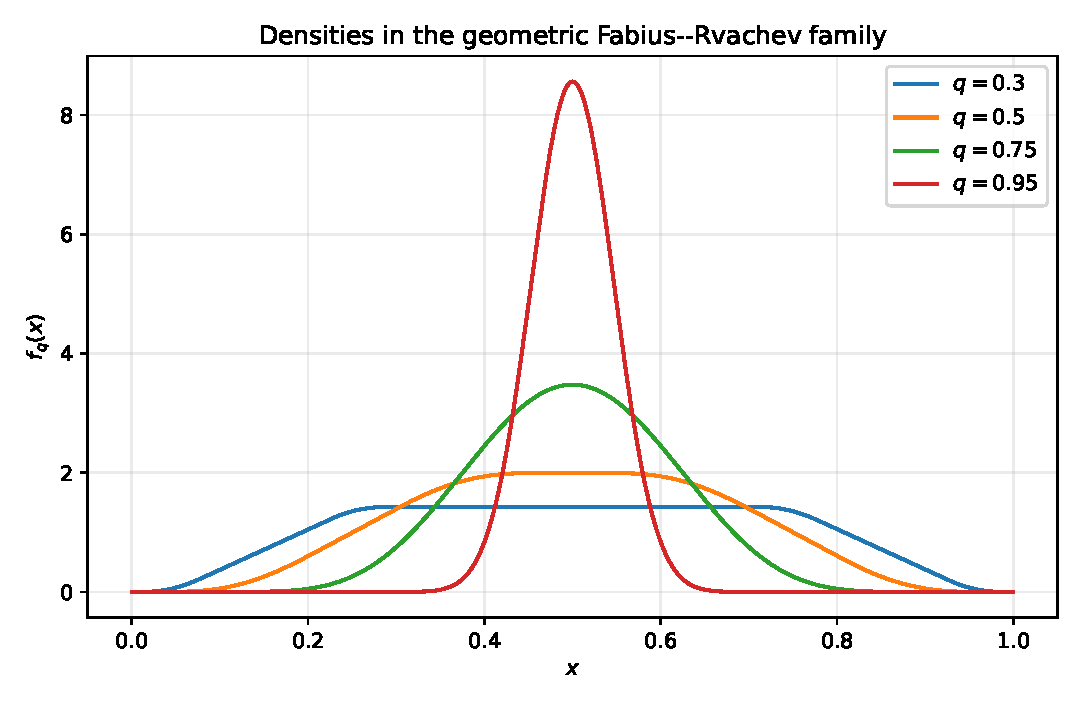
\includegraphics[width=0.92\textwidth]{q_family_densities.pdf}
\caption{Deterministic fixed-point approximations of $f_q$.  The exact plateau for $q=0.30$
ends at $x=q$ and $x=1-q$.  At $q=1/2$ the plateau collapses to a point; for larger $q$ the
law becomes sharply concentrated and strictly unimodal.}
\label{fig:q-densities}
\end{figure}

\section{Gaussian degeneration and an Edgeworth frontier}
\label{sec:gaussian}

Let
\[
 G_q=\frac{Z_q}{\sigma_q},
 \qquad \sigma_q^2=\frac{1-q}{12(1+q)}.
\]
The largest normalized summand has magnitude of order $\sqrt{1-q}$, while the total variance
is one.  This is a triangular-array central-limit regime.

\begin{theorem}[Gaussian limit]
\label{thm:clt}
As $q\uparrow1$,
\begin{equation}
 G_q\ \xrightarrow{\ d\ }\ \Normal(0,1).                    \label{eq:clt}
\end{equation}
The standardized even cumulants are
\begin{equation}
 \gamma_{2m}(q):=\kappa_{2m}(G_q)
 =\frac{B_{2m}}{2m}12^m
   \frac{(1-q^2)^m}{1-q^{2m}}.                               \label{eq:standard-cumulants}
\end{equation}
In particular,
\begin{align}
 \gamma_4(q)&=-\frac65\frac{1-q^2}{1+q^2},                  \label{eq:gamma4}\\
 \gamma_6(q)&=\frac{48}{7}\frac{(1-q^2)^2}{1+q^2+q^4}.      \label{eq:gamma6}
\end{align}
For every fixed $T<\infty$, uniformly for $|t|\le T$,
\begin{equation}
 \log\E\e^{\ii tG_q}
 =-\frac{t^2}{2}+\frac{\gamma_4(q)t^4}{4!}
  +\bigO_T\bigl((1-q)^2\bigr).                              \label{eq:compact-edgeworth}
\end{equation}
\end{theorem}

\begin{proof}
Write
\[
 G_q=\sum_{j\ge0}\alpha_{q,j}(U_j-\tfrac12),
 \qquad
 \alpha_{q,j}=\frac{cq^j}{\sigma_q}.
\]
The summands are bounded, their variances sum to one, and
\[
 \max_j|\alpha_{q,j}|=\frac{c}{\sigma_q}
 =\sqrt{12(1-q)(1+q)}\longrightarrow0.
\]
The Lindeberg condition is therefore immediate, proving \eqref{eq:clt}.
Dividing \eqref{eq:q-cumulants} by $\sigma_q^{2m}$ gives
\eqref{eq:standard-cumulants}; elementary factorization gives
\eqref{eq:gamma4}--\eqref{eq:gamma6}.

For the compact-frequency expansion, expand the logarithm of each sinc factor.  The maximum
factor argument is $\bigO_T(\sqrt{1-q})$, so the expansion is uniform.  The quadratic terms
sum to $-t^2/2$, the quartic terms sum to $\gamma_4t^4/4!$, and the sum of all terms of order
six and higher is $\bigO_T((1-q)^2)$ because
$\gamma_{2m}(q)=\bigO((1-q)^{m-1})$ for $m\ge3$.
\end{proof}

Formally inverting \eqref{eq:compact-edgeworth} suggests
\begin{equation}
 \sigma_q f_q\!\left(\frac12+\sigma_qx\right)
 =\varphi(x)\left[1+\frac{\gamma_4(q)}{24}\He_4(x)\right]
 +\bigO((1-q)^2),                                            \label{eq:edgeworth-formal}
\end{equation}
where
\(
 \varphi(x)=(2\pi)^{-1/2}\e^{-x^2/2}
\)
and $\He_4(x)=x^4-6x^2+3$.
At the center this predicts
\begin{equation}
 f_q(1/2)
 =\frac{1}{\sqrt{2\pi}\sigma_q}
  \left[1+\frac{\gamma_4(q)}8+\bigO((1-q)^2)\right].        \label{eq:center-edgeworth}
\end{equation}
For $q=0.95$, the deterministic computation gives $f_q(1/2)=8.56266675$, while the Gaussian
term with the quartic correction gives $8.56$ to the displayed precision.

\begin{conjecture}[Uniform density Edgeworth expansion]
\label{conj:edgeworth}
For every fixed integer $r\ge1$, the normalized density of $G_q$ admits a uniform all-orders
Edgeworth expansion through order $(1-q)^r$, with coefficients obtained by Bell contraction
of the explicit standardized cumulants \eqref{eq:standard-cumulants}.  In particular,
\eqref{eq:edgeworth-formal} holds uniformly in $x\in\R$ with error
$\bigO((1-q)^2)$ after inclusion of the complete order-$(1-q)^2$ Hermite polynomial.
\end{conjecture}

The missing ingredient is not the coefficient algebra, which is explicit, but a clean
$q$-uniform Fourier-tail estimate strong enough to justify termwise inversion on the whole
line.

\begin{figure}[ht]
\centering
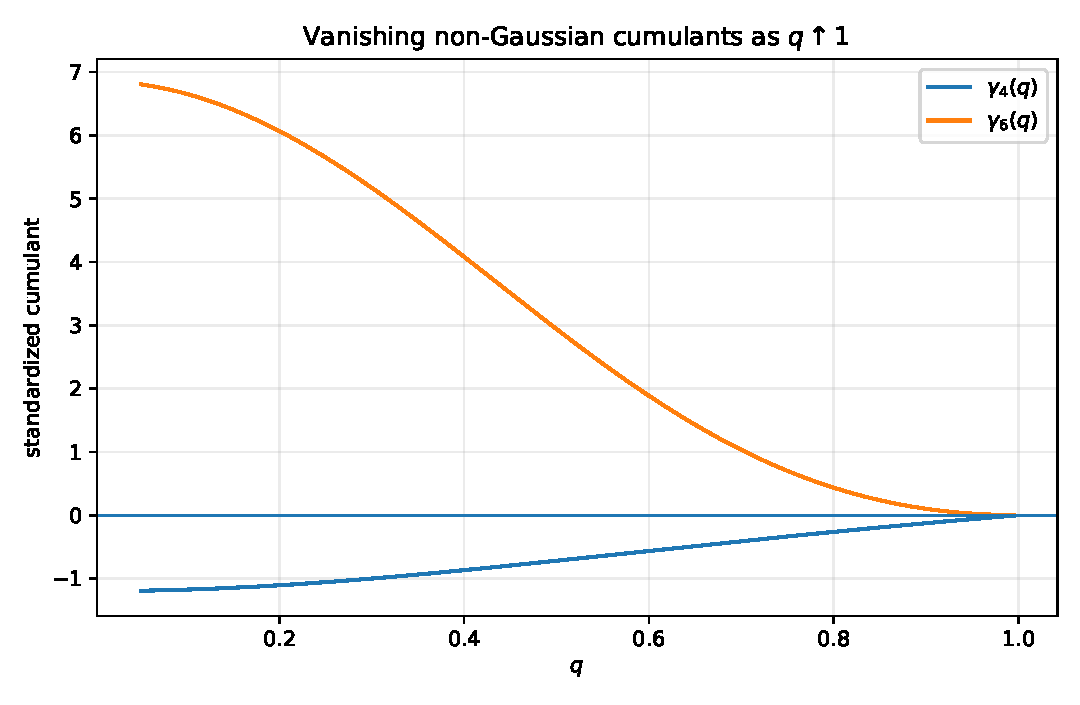
\includegraphics[width=0.86\textwidth]{standardized_cumulants.pdf}
\caption{The exact standardized cumulants $\gamma_4(q)$ and $\gamma_6(q)$.  Their decay to
zero quantifies the Gaussian degeneration as $q\uparrow1$.}
\label{fig:cumulants}
\end{figure}

\section{A rigorous endpoint law and Lambert-\texorpdfstring{$W$}{W} inversion}
\label{sec:endpoint}

The exact dyadic repository contains a much sharper lower-Lambert expansion with periodic
corrections.  The purpose here is different: establish, for every $q$, the first two universal
logarithmic scales by a short probability argument, then invert them rigorously.  Set
\[
 L=\log(1/x),
 \qquad a=\log(1/q).
\]

\subsection{Finite-simplex upper bound}

For $n\ge1$, let
\[
 S_n=c\sum_{j=0}^{n-1}q^jU_j.
\]
If $0<x\le cq^{n-1}$, then the simplex
\(
 \sum_{j<n}cq^ju_j\le x
\)
lies entirely inside the unit cube.  Its volume is exact:
\begin{equation}
 \Prob(S_n\le x)
 =\frac{x^n}{n!c^nq^{n(n-1)/2}}.                            \label{eq:simplex-volume}
\end{equation}
Since $X_q\ge S_n$, this is an upper bound for $F_q(x)$.

\subsection{A matching product lower bound}

Choose $n$ so that the deterministic tail is at most $x/2$:
\[
 c\sum_{j=n}^{\infty}q^j=q^n\le x/2.
\]
If, for every $0\le j<n$,
\[
 U_j\le\frac{x}{2ncq^j},
\]
then the first $n$ summands contribute at most $x/2$, and hence $X_q\le x$.  For small $x$
the displayed thresholds are all at most one, giving the lower bound
\begin{equation}
 F_q(x)
 \ge\frac{x^n}{(2nc)^nq^{n(n-1)/2}}.                        \label{eq:product-lower}
\end{equation}

\begin{theorem}[Two-term logarithmic endpoint law]
\label{thm:endpoint}
For each fixed $q\in(0,1)$, as $x\downarrow0$,
\begin{equation}
 \boxed{\displaystyle
 \log F_q(x)
 =-\frac{L^2}{2a}-\frac{L\log L}{a}+\bigO_q(L),
 \qquad L=\log(1/x),\quad a=\log(1/q).}                     \label{eq:endpoint-main}
\end{equation}
By symmetry, the same law holds for $1-F_q(1-x)$.
\end{theorem}

\begin{proof}
For the upper bound, choose
\[
 n_+(x)=\left\lfloor\frac{L+\log c}{a}\right\rfloor+1.
\]
Then $x\le cq^{n_+-1}$, so \eqref{eq:simplex-volume} applies.  Taking logarithms gives
\begin{equation}
 \log F_q(x)
 \le-n_+L-\log(n_+!)-n_+\log c+\frac{a}{2}n_+(n_+-1).       \label{eq:upper-log}
\end{equation}
Since $n_+=L/a+\bigO_q(1)$, Stirling's formula yields
\[
 -n_+L+\frac{a}{2}n_+^2=-\frac{L^2}{2a}+\bigO_q(L),
 \qquad
 -\log(n_+!)=-\frac{L\log L}{a}+\bigO_q(L).
\]
Thus the right side of \eqref{eq:upper-log} is
\[
 -\frac{L^2}{2a}-\frac{L\log L}{a}+\bigO_q(L).
\]

For the lower bound, take
\[
 n_-(x)=\left\lceil\frac{\log(2/x)}{a}\right\rceil.
\]
Then $q^{n_-}\le x/2$.  The ceiling relation also gives
$q^{n_--1}>x/2$, so the largest threshold in the product event is at most
$1/(n_-c)$ and is therefore below one for sufficiently small $x$.  Apply
\eqref{eq:product-lower} and take logarithms:
\begin{equation}
 \log F_q(x)
 \ge-n_-L-n_-\log(2n_-c)+\frac{a}{2}n_-(n_--1).             \label{eq:lower-log}
\end{equation}
Again $n_-=L/a+\bigO_q(1)$, so the quadratic terms contribute
$-L^2/(2a)+\bigO_q(L)$ and the $-n_-\log n_-$ term contributes
$-(L\log L)/a+\bigO_q(L)$.  The upper and lower bounds match at the two displayed scales.
\end{proof}

\begin{remark}[Why the second term is already nontrivial]
The quadratic term comes from balancing the small probability of constraining roughly
$L/a$ coordinates against the geometric Jacobian $q^{n(n-1)/2}$.  The additional
$-L\log L/a$ term is the factorial entropy of the finite simplex (upper bound) and the
$n^{-n}$ cost of a balanced coordinate allocation (lower bound).  Thus the second scale is
not an artifact of saddle notation; it is forced by elementary high-dimensional geometry.
\end{remark}

\subsection{Inverse endpoint law}

Let $Q_q(y)=F_q^{-1}(y)$ for $0<y<1$, and put
\[
 Y=\log(1/y),
 \qquad
 L_y=\log\frac{1}{Q_q(y)},
 \qquad
 S=\sqrt{2aY}.
\]
Equation \eqref{eq:endpoint-main} is equivalent to
\begin{equation}
 2aY=L_y^2+2L_y\log L_y+\bigO_q(L_y).                        \label{eq:inverse-prep}
\end{equation}
Since $(\log L_y)^2=\smallo(L_y)$, one obtains
\[
 S=L_y+\log L_y+\bigO_q(1).
\]
The inverse of $r\mapsto r+\log r$ is $r=W(\e^s)$.

\begin{corollary}[Lambert-$W$ quantile law]
\label{cor:inverse-endpoint}
As $y\downarrow0$,
\begin{align}
 \boxed{\displaystyle
 \log\frac1{Q_q(y)}
 =W\!\left(\exp\sqrt{2a\log(1/y)}\right)+\bigO_q(1)}        \label{eq:inverse-W}\\
 &=\sqrt{2a\log(1/y)}
   -\frac12\log\!\bigl(2a\log(1/y)\bigr)+\bigO_q(1).       \label{eq:inverse-expanded}
\end{align}
The corresponding upper-end quantile follows from symmetry:
$Q_q(1-y)=1-Q_q(y)$.
\end{corollary}

\begin{proof}
From \eqref{eq:inverse-prep},
\[
 S^2=(L_y+\log L_y)^2+\bigO_q(L_y),
\]
so $S=L_y+\log L_y+\bigO_q(1)$.  If $r+\log r=s$, then
$r\e^r=\e^s$ and $r=W(\e^s)$.  Since the derivative of $r+\log r$ is bounded away from zero
for large $r$, the additive $\bigO_q(1)$ perturbation in $s$ changes $r$ by
$\bigO_q(1)$.  This proves \eqref{eq:inverse-W}.  The standard large-argument expansion
$W(\e^S)=S-\log S+\bigO((\log S)/S)$ gives \eqref{eq:inverse-expanded}.
\end{proof}

This is deliberately weaker than the repository's all-orders dyadic lower-Lambert machinery,
but it is rigorous for every $q$ and directly links the inverse Fabius scale to Lambert $W$.

\begin{figure}[ht]
\centering
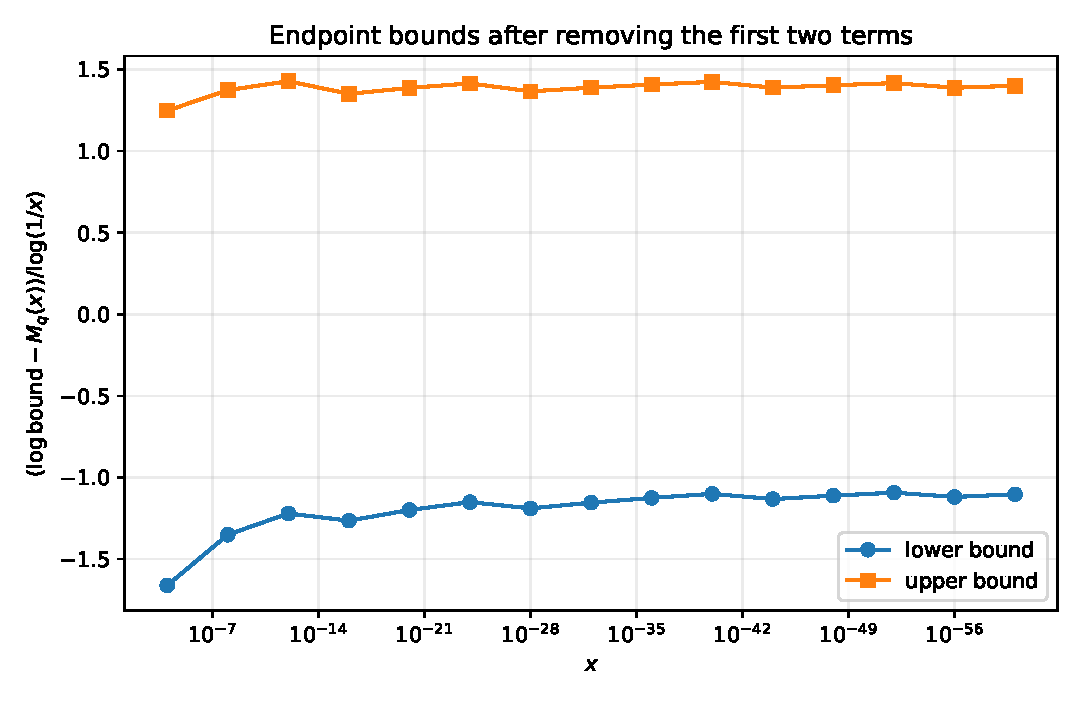
\includegraphics[width=0.88\textwidth]{endpoint_bound_residuals.pdf}
\caption{For $q=1/2$, the rigorous upper and lower logarithmic bounds after subtracting the
two universal terms and dividing by $L$.  Bounded residuals are exactly what
\Cref{thm:endpoint} predicts.}
\label{fig:endpoint-bounds}
\end{figure}

\subsection{The expected periodic completion}

The Laplace transform is
\begin{equation}
 \mathcal L_q(s)=\E\e^{-sX_q}
 =\prod_{j=0}^{\infty}\frac{1-\e^{-csq^j}}{csq^j}.          \label{eq:laplace-product}
\end{equation}
It is a harmonic sum over the logarithmic lattice $\log s-ja$.  Mellin analysis of such
sums normally produces a polynomial in the logarithmic scale plus a periodic function of its
fractional part \cite{flajolet1995}.  This mechanism is exactly what occurs in the dyadic
endpoint expansion already present in the repository.

\begin{conjecture}[Full geometric endpoint transseries]
\label{conj:q-transseries}
For every fixed $q\in(0,1)$ there exists a natural lower-Lambert saddle coordinate
$\lambda_q(x)\to\infty$ and smooth $1$-periodic functions
$A_{q,r}:\R/\Z\to\R$ such that
\begin{equation}
 F_q(x)
 =\exp\bigl(-\mathcal S_q(\lambda_q(x))\bigr)
  \lambda_q(x)^{-1/2}
  \left[
   A_{q,0}(\{\lambda_q(x)\})
   +\sum_{r=1}^{N}\frac{A_{q,r}(\{\lambda_q(x)\})}{\lambda_q(x)^r}
   +\bigO_{q,N}(\lambda_q^{-N-1})
  \right],                                                  \label{eq:q-transseries}
\end{equation}
where $\mathcal S_q$ has an explicit expansion whose first two consequences are
\eqref{eq:endpoint-main}.  The leading periodic amplitude $A_{q,0}$ is positive and
nonconstant for generic $q$.
\end{conjecture}

\begin{problem}[Fourier modes of the endpoint phase]
Determine the Mellin-residue formula for the Fourier coefficients of $A_{q,0}$ and classify
those $q$ for which one or more nonzero modes vanish.  The dyadic development suggests
nonvanishing, but the free parameter may admit exceptional arithmetic ratios.
\end{problem}

\section{Fourier-zero arithmetic and the special role of base two}
\label{sec:zeros}

The product \eqref{eq:phi-y} makes the zero set explicit:
\begin{equation}
 \mathcal Z_q
 =\left\{\frac{\pi k}{cq^j}: k\in\Z\setminus\{0\},\ j\ge0\right\}. \label{eq:zero-set}
\end{equation}
Each individual factor has a simple nonzero zero.  Multiplicity therefore counts collisions
between geometric scales.

\begin{theorem}[Reciprocal-integer multiplicities]
\label{thm:zero-multiplicity}
Let $q=1/b$ with an integer $b\ge2$.  Then every nonzero zero of $\widehat u_q$ lies on the
lattice
\begin{equation}
 t=\frac{\pi N}{1-1/b},\qquad N\in\Z\setminus\{0\}.          \label{eq:zero-lattice}
\end{equation}
Its multiplicity is
\begin{equation}
 \boxed{\displaystyle
 \operatorname{mult}\!\left(\frac{\pi N}{1-1/b}\right)
 =1+v_b(|N|),}                                               \label{eq:zero-mult}
\end{equation}
where
\(
 v_b(N)=\max\{r\ge0:b^r\mid N\}
\)
uses divisibility by the whole base $b$, which need not be prime.
\end{theorem}

\begin{proof}
At $q=1/b$, the $j$th factor is
$\sinc(cb^{-j}t)$.  At $t=\pi N/c$, it vanishes exactly when
$b^j\mid N$.  Thus the vanishing factors are indexed by
$j=0,1,\ldots,v_b(|N|)$, and their simple multiplicities add.  Conversely, every zero of the
$j$th factor has the form $t=\pi kb^j/c=\pi N/c$ for an integer $N\ne0$.
\end{proof}

For the classical up-function $b=2$, the zeros are at $2\pi N$ in the convention
\eqref{eq:phi-y}, with multiplicity $1+v_2(N)$.

\begin{proposition}[Generic simplicity criterion]
\label{prop:generic-zeros}
If $q^d\notin\Q$ for every integer $d\ge1$, then every nonzero zero of
$\widehat u_q$ is simple.
\end{proposition}

\begin{proof}
A collision between scales $j<k$ would give
\[
 \frac{k_1}{q^j}=\frac{k_2}{q^k}
 \quad\Longrightarrow\quad
 q^{k-j}=\frac{k_2}{k_1}\in\Q
\]
for nonzero integers $k_1,k_2$, contrary to the hypothesis.
\end{proof}

\begin{problem}[Complete collision classification]
For algebraic $q$ such that $q^d\in\Q$ for some $d$, describe the zero set as a union of
arithmetic lattices with a closed multiplicity formula.  The reciprocal-integer theorem is
the cleanest case; rational $q=r/s$ and radical rational $q=(r/s)^{1/d}$ should lead to a
finite-state valuation problem.
\end{problem}

\subsection{Why the contiguous Thue--Morse block is uniquely dyadic}

For an integer base $b\ge2$, consider the finite product
\begin{equation}
 P_{b,N}(z)=\prod_{j=0}^{N-1}(1-z^{b^j}).                    \label{eq:b-product}
\end{equation}
Expanding by subsets gives
\begin{equation}
 P_{b,N}(z)
 =\sum_{\varepsilon\in\{0,1\}^N}
  (-1)^{\varepsilon_0+\cdots+\varepsilon_{N-1}}
  z^{\varepsilon_0+\varepsilon_1b+\cdots+\varepsilon_{N-1}b^{N-1}}. \label{eq:b-expansion}
\end{equation}

\begin{proposition}[Dyadic contiguity]
\label{prop:dyadic-contiguity}
The exponents in \eqref{eq:b-expansion} form a complete interval of consecutive integers if
and only if $b=2$.  In that case,
\begin{equation}
 P_{2,N}(z)=\sum_{n=0}^{2^N-1}(-1)^{\wt(n)}z^n,              \label{eq:tm-block}
\end{equation}
which is the contiguous signed Thue--Morse block.  For every $b\ge3$, the exponents are
precisely the integers whose first $N$ base-$b$ digits belong to $\{0,1\}$; they form a
sparse Cantor-type set with gaps.
\end{proposition}

\begin{proof}
For $b=2$, binary expansion is a bijection between $\{0,1\}^N$ and
$\{0,1,\ldots,2^N-1\}$, and the subset size is the binary digit sum.  If $b\ge3$, the integer
$2$ is absent already at the first digit, while $0$ and $1$ are present, so the exponent set
is not contiguous.  The stated digit characterization is immediate from
\eqref{eq:b-expansion}.
\end{proof}

This gives a structural explanation for a feature that can otherwise look accidental.  The
reciprocal-integer Fourier products exist for every base $b$, and their zero multiplicities
are controlled by $v_b$.  But only $b=2$ makes the subset-product coefficients occupy every
integer index.  The Thue--Morse sequence is therefore not merely one member of a uniform
$b$-adic family; it is the unique no-gap member.

\begin{problem}[Sparse $b$-adic signed operators]
For $b\ge3$, develop the analogue of the dyadic signed extension on the sparse digit set
$\{0,1\}$ in base $b$.  Natural questions include transfer matrices for rarefied sums,
operator spectra, exact cancellation order, and whether the missing digits can be supplied by
multinomial factors to produce a different automatic sequence with a contiguous block.
\end{problem}

\section{Phase-aware Lagrange and Richardson extrapolation}
\label{sec:phase}

The dyadic corpus already contains two ingredients that should not be conflated:
geometric-node Lagrange extraction and $q$-Richardson cancellation of errors such as
$2^{-rn}$.  Endpoint saddle expansions introduce a different obstacle: coefficients depend
periodically on the fractional part of a Lambert variable.  Ordinary extrapolation across
samples with different phases mixes different coefficient functions and can lose its nominal
order.  The cure is to move by integer increments in the Lambert variable.

\subsection{A phase-preserving interpolation theorem}

Let $u\in\R/\Z$ be fixed.  Suppose an observable has the phase-class representation
\begin{equation}
 R(\lambda)=L+h_u(1/\lambda),
 \qquad \lambda\equiv u\pmod1,                               \label{eq:phase-model}
\end{equation}
where $h_u$ is smooth near zero and $h_u(0)=0$.  Use the samples
$\lambda_m=\lambda+m$, $m=0,\ldots,p$; all have the same fractional phase.

\begin{theorem}[Phase-aware Lagrange filter]
\label{thm:phase-lagrange}
For $m=0,\ldots,p$, define
\begin{equation}
 w_m^{(p)}(\lambda)
 =(-1)^{p-m}\frac{(\lambda+m)^p}{m!(p-m)!}.                  \label{eq:phase-weights}
\end{equation}
Then
\begin{align}
 \sum_{m=0}^{p}w_m^{(p)}(\lambda)&=1,                       \label{eq:weights-sum}\\
 \sum_{m=0}^{p}\frac{w_m^{(p)}(\lambda)}{(\lambda+m)^r}&=0
 \qquad(1\le r\le p),                                      \label{eq:weights-kill}
\end{align}
and
\begin{equation}
 \sum_{m=0}^{p}w_m^{(p)}(\lambda)R(\lambda+m)
 =L+\bigO_{u,p}(\lambda^{-p-1}).                             \label{eq:phase-accelerated}
\end{equation}
More precisely, if $h_u\in C^{p+1}[0,1/\lambda]$, then the error is bounded by
\begin{equation}
 \frac{\|h_u^{(p+1)}\|_\infty}{(p+1)!}
 \prod_{m=0}^{p}\frac{1}{\lambda+m}.                        \label{eq:phase-error}
\end{equation}
\end{theorem}

\begin{proof}
Interpolate $h_u(t)$ at the nodes
$t_m=(\lambda+m)^{-1}$ and evaluate the degree-$p$ interpolant at $t=0$.  The Lagrange basis
weight is
\[
 \ell_m(0)=\prod_{r\ne m}\frac{-t_r}{t_m-t_r}.
\]
Since
\[
 t_m-t_r=\frac{r-m}{(\lambda+m)(\lambda+r)},
\]
a direct cancellation gives
\[
 \ell_m(0)
 =(-1)^{p-m}\frac{(\lambda+m)^p}{m!(p-m)!},
\]
which is \eqref{eq:phase-weights}.  Exactness on $1,t,\ldots,t^p$ gives
\eqref{eq:weights-sum}--\eqref{eq:weights-kill}.  The standard interpolation remainder at
zero is
\[
 \frac{h_u^{(p+1)}(\xi)}{(p+1)!}\prod_{m=0}^{p}(0-t_m),
\]
which proves \eqref{eq:phase-error} and hence \eqref{eq:phase-accelerated}.
\end{proof}

\begin{remark}[Conditioning]
The weights grow individually like $\lambda^p$ and cancel strongly.  The theorem is exact,
but a floating-point implementation should use extended precision, compensated summation,
or a barycentric form.  The deterministic experiment in \Cref{sec:numerics} uses moderate
orders and directly verifies the predicted slope.
\end{remark}

\subsection{Fourier phase averaging}

A complementary operation removes periodic modes rather than preserving a single phase.

\begin{theorem}[Root-of-unity phase filter]
\label{thm:phase-average}
Let
\(
 \Psi(u)=\sum_{k\in\Z}c_k\e^{2\pi\ii ku}
\)
be an absolutely convergent Fourier series.  Then
\begin{equation}
 \frac1M\sum_{r=0}^{M-1}\Psi\!\left(u+\frac rM\right)
 =\sum_{\ell\in\Z}c_{\ell M}\e^{2\pi\ii\ell Mu}.            \label{eq:phase-average}
\end{equation}
If $|c_k|\le C\e^{-\rho|k|}$, then
\begin{equation}
 \left|
 \frac1M\sum_{r=0}^{M-1}\Psi\!\left(u+\frac rM\right)-c_0
 \right|
 \le\frac{2C\e^{-\rho M}}{1-\e^{-\rho M}}.                 \label{eq:phase-average-error}
\end{equation}
\end{theorem}

\begin{proof}
Insert the Fourier series and use
\[
 \frac1M\sum_{r=0}^{M-1}\e^{2\pi\ii kr/M}
 =\begin{cases}1,&M\mid k,\\0,&M\nmid k.\end{cases}
\]
The error bound is the geometric sum over nonzero multiples of $M$.
\end{proof}

The two filters answer different questions.  Phase-preserving Lagrange interpolation recovers
the limit while keeping all periodic coefficients fixed.  Root-of-unity averaging projects a
periodic coefficient onto the Fourier modes divisible by $M$, converging exponentially to its
mean when the phase function is analytic in a strip.

\subsection{Exact Lambert-\texorpdfstring{$W$}{W} sample nodes}

Suppose the relevant endpoint coordinate satisfies
\begin{equation}
 x=(\lambda+\beta)\e^{-a\lambda},                            \label{eq:lambert-node-equation}
\end{equation}
with $a>0$.  Then
\begin{equation}
 \boxed{\displaystyle
 \lambda=-\beta-\frac1a
 W_{-1}\!\left(-ax\e^{-a\beta}\right),}                    \label{eq:lambert-node-inverse}
\end{equation}
where the lower branch is selected for large positive $\lambda$.  Conversely, once a starting
phase $\lambda\equiv u\pmod1$ is chosen, the phase-locked physical nodes are
\begin{equation}
 x_m=(\lambda+m+\beta)\e^{-a(\lambda+m)},
 \qquad m=0,\ldots,p.                                       \label{eq:physical-nodes}
\end{equation}
Their ratio is
\begin{equation}
 \frac{x_{m+1}}{x_m}
 =q\frac{\lambda+m+1+\beta}{\lambda+m+\beta},               \label{eq:node-ratio}
\end{equation}
so they are asymptotically geometric but carry exactly the correction needed to preserve the
Lambert phase.

\subsection{A practical composite algorithm}

A numerically robust endpoint study can use the following sequence.

\begin{algorithm}[Phase-resolved endpoint extraction]
\label{alg:phase}
Given an observable $R(x)$ believed to have a periodic lower-Lambert expansion:
\begin{enumerate}
\item derive or fit the monotone saddle map $x\leftrightarrow\lambda$ and choose a phase
      $u\in[0,1)$;
\item select a large $\lambda\equiv u\pmod1$ and generate $x_m$ from
      \eqref{eq:physical-nodes};
\item evaluate $R(x_m)$ at increased precision;
\item apply the weights \eqref{eq:phase-weights} in barycentric or compensated form;
\item repeat for several $u$ to reconstruct the periodic coefficient functions;
\item optionally average $M$ equally spaced phases and use \eqref{eq:phase-average} to isolate
      the mean or selected Fourier harmonics.
\end{enumerate}
\end{algorithm}

This is a synthesis of Lambert inversion, Lagrange interpolation, Richardson cancellation,
and Fourier projection, but its exact weight formula and fixed-phase error theorem are not the
same as the repository's existing geometric-grid filter.

\begin{figure}[ht]
\centering
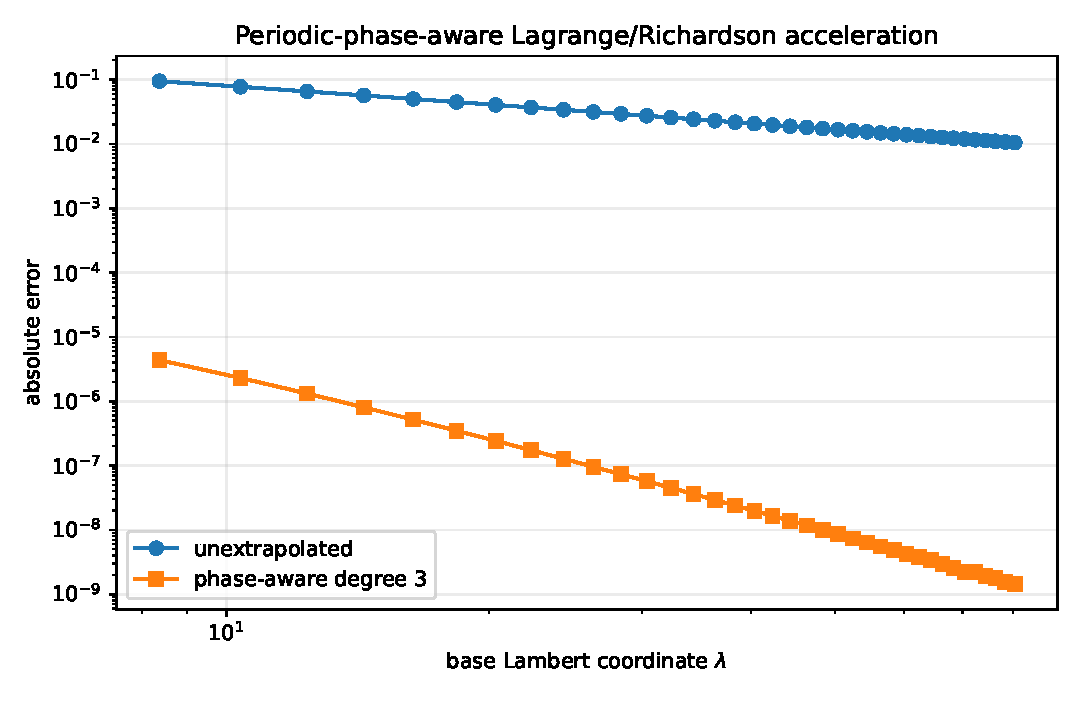
\includegraphics[width=0.88\textwidth]{phase_aware_extrapolation.pdf}
\caption{A synthetic periodic-phase model used only to verify
\Cref{thm:phase-lagrange}.  The raw error has slope approximately $-1$; a degree-three
phase-preserving filter has observed slope approximately $-3.82$, approaching the predicted
$-4$.  This experiment does not assume or fit the unknown endpoint coefficients of $F_q$.}
\label{fig:phase-extrapolation}
\end{figure}

\section{Deterministic numerical experiments}
\label{sec:numerics}

The companion program \texttt{numerical\_experiments.py} uses no Monte Carlo sampling.  It is
intended to test consequences of proved identities and to provide reconnaissance for the
conjectures.

\subsection{Fixed-point density solver}

Starting from the uniform density, the code repeatedly applies the distributional fixed-point
operator.  On a uniform grid it computes a CDF by trapezoidal integration and then updates
\[
 f^{\mathrm{new}}(x)
 =\frac{F^{\mathrm{old}}(x/q)-F^{\mathrm{old}}((x-c)/q)}{c}.
\]
The density is renormalized after each step, and convergence is measured in the sup norm.
The output verifies mass, symmetry, and the exact plateau.  Representative results are shown
in \Cref{tab:numerical-density}.

\begin{table}[ht]
\centering
\caption{Fixed-point density diagnostics.}
\label{tab:numerical-density}
\begin{tabular}{@{}rrrrr@{}}
\toprule
$q$ & iterations & mass error & symmetry error & $f_q(1/2)$\\
\midrule
$0.30$ & $11$  & $2.2\cdot10^{-16}$ & $1.2\cdot10^{-15}$ & $1.42857142857$\\
$0.50$ & $19$  & $0$                & $4.2\cdot10^{-15}$ & $2.00000000000$\\
$0.75$ & $45$  & $0$                & $9.2\cdot10^{-14}$ & $3.47864814200$\\
$0.95$ & $247$ & $0$                & $2.6\cdot10^{-12}$ & $8.56266675023$\\
\bottomrule
\end{tabular}
\end{table}

For $q=0.30$, the theoretical plateau height is $1/(1-q)=10/7$, and the maximum interior
grid error on $[q,1-q]$ was exactly zero at machine precision.

\subsection{Cumulant checks}

The script computes standardized cumulants both from the general Bernoulli formula and from
the simplified rational expressions.  The differences were at most machine roundoff.  For
example,
\begin{center}
\begin{tabular}{@{}rrrr@{}}
\toprule
$q$ & $\sigma_q^2$ & $\gamma_4(q)$ & $\gamma_6(q)$\\
\midrule
$0.25$ & $0.0500000$ & $-1.0588235$ & $5.6514914$\\
$0.50$ & $0.0277778$ & $-0.7200000$ & $2.9387755$\\
$0.75$ & $0.0119048$ & $-0.3360000$ & $0.6985447$\\
$0.90$ & $0.0043860$ & $-0.1259669$ & $0.1003783$\\
$0.97$ & $0.0012690$ & $-0.0365397$ & $0.0084745$\\
\bottomrule
\end{tabular}
\end{center}
The rapid decrease of higher standardized cumulants supports the Edgeworth program.

\subsection{Endpoint bounds}

For $q=1/2$ and $x$ from $10^{-4}$ down to $10^{-60}$, the program evaluates the exact
logarithms of the finite-simplex upper bound and balanced-product lower bound.  After adding
$L^2/(2a)+(L\log L)/a$ and dividing by $L$, both residuals remain bounded, as displayed in
\Cref{fig:endpoint-bounds}.  This is a numerical visualization of a theorem rather than an
independent fit.

\subsection{Phase-aware extrapolation}

The synthetic model is
\[
 R(\lambda)=L+\frac{a_1(u)}{\lambda}
              +\frac{a_2(u)}{\lambda^2}
              +\frac{a_3(u)}{\lambda^3}
              +\frac{a_4(u)}{\lambda^4},
 \qquad u=\{\lambda\},
\]
with trigonometric coefficient functions.  Sampling at $\lambda,\lambda+1,\lambda+2,
\lambda+3$ holds $u$ fixed.  A log--log regression gave raw slope $-0.990967$ and accelerated
slope $-3.824509$; the latter tends to $-4$ as the asymptotic range and precision increase.

\subsection{Zero multiplicities}

For $b=2,3,4,5$ and $1\le|N|\le64$, the code enumerates vanishing sinc factors and verifies
\(
 \operatorname{mult}=1+v_b(N)
\)
without exception.  This check is elementary but guards against an easy normalization error
in the lattice spacing.

\subsection{Reproducibility}

Running
\begin{lstlisting}[style=code]
python3 numerical_experiments.py
\end{lstlisting}
from the report directory regenerates the four PDF figures, a CSV summary, and the text log.
The script contains detailed comments, parameter checks, deterministic stopping criteria, and
no external data dependency.

\section{Conjectures and promising research directions}
\label{sec:future}

This section collects the most promising next steps in a form designed to be falsifiable and,
where possible, formalizable.

\subsection{Analytic shape}

\begin{conjecture}[Strict log-concavity]
For $q>1/2$, the density $f_q$ is strictly log-concave on $(0,1)$.  Equivalently,
\[
 f_q(\theta x+(1-\theta)y)
 >f_q(x)^\theta f_q(y)^{1-\theta}
\]
for distinct $x,y\in(0,1)$ and $0<\theta<1$.
\end{conjecture}

The exact plateau theorem shows that $q=1/2$ is the only possible transition value.  A proof
would likely combine equality cases in Pr\'ekopa--Leindler with the self-similar decomposition
and the fact that no single interval dominates the remaining support when $q>1/2$.

\begin{problem}[Monotonicity of the peak]
Prove or disprove that $q\mapsto f_q(1/2)$ is strictly increasing.  Convex-order contraction
suggests the statement but does not imply pointwise density order.  The Gaussian prediction is
\[
 f_q(1/2)\sim\sqrt{\frac{6(1+q)}{\pi(1-q)}}.
\]
\end{problem}

\subsection{Uniform Gaussian asymptotics}

\begin{conjecture}[All-orders Edgeworth expansion]
The expansion in \Cref{conj:edgeworth} holds uniformly with explicit coefficients generated by
\eqref{eq:standard-cumulants}.  In particular,
\[
 f_q(1/2)
 =\frac{1}{\sqrt{2\pi}\sigma_q}
  \left(1-\frac{3}{20}(1-q)+\bigO((1-q)^2)\right).
\]
\end{conjecture}

A promising proof strategy is to split the normalized Fourier integral at
$|t|=(1-q)^{-\eta}$, use the cumulant expansion on the central range, and exploit a block of
roughly $(1-q)^{-1}$ sinc factors for a $q$-uniform tail majorant.

\subsection{Endpoint phase and inverse transfer}

\begin{conjecture}[Nonconstant periodic amplitude]
For generic $q$, the leading phase function $A_{q,0}$ in
\eqref{eq:q-transseries} is nonconstant, real analytic, and has no vanishing nonzero Fourier
coefficient.  Exceptional $q$, if any, form a thin arithmetic set.
\end{conjecture}

\begin{conjecture}[Inverse phase transfer]
Let $Q_q=F_q^{-1}$.  The periodic endpoint functions of $F_q$ transfer to a complete expansion
of $Q_q(y)$ through the lower branch $W_{-1}$ and formal Lagrange inversion.  The phase of the
inverse is not simply the phase of $\log(1/y)$; it includes the derivative of the saddle map
and a computable phase shift from the leading amplitude.
\end{conjecture}

The phase-aware sampling theorem provides a practical way to distinguish these possibilities
numerically without averaging the phase away.

\subsection{A two-parameter large-deviation/Gaussian phase diagram}

The limits $x\downarrow0$ and $q\uparrow1$ do not commute.  For fixed $q$, the endpoint law is
quadratic in $\log(1/x)$.  For $q\uparrow1$ at the central scale
$x=1/2+\sigma_qz$, the law is Gaussian.  Between them lies a double-scaling region.

\begin{problem}[Joint scaling]
Determine a uniform asymptotic for
\[
 \Prob\!\left(X_q\le\frac12-r_q\right)
\]
when $q\uparrow1$ and $r_q/\sigma_q\to\infty$ while $r_q<1/2$.  Identify the transition from
the Gaussian rate $r_q^2/(2\sigma_q^2)$ to the logarithmic endpoint action of
\Cref{thm:endpoint}.  A natural tool is the exact cumulant generating product
\eqref{eq:mgf-product} and a saddle that moves through the geometric scale lattice.
\end{problem}

\subsection{Arithmetic zero collisions}

\begin{problem}[Algebraic collision graph]
For algebraic $q$, define a graph on scales $j\ge0$ by joining $j$ and $k$ when
$q^{|j-k|}\in\Q$.  Express Fourier-zero multiplicities in terms of rational valuations along
connected components.  Determine when the multiplicity function is automatic or regular in
the sense of Allouche--Shallit.
\end{problem}

\subsection{Beyond binary Thue--Morse}

\begin{problem}[Contiguous completion in higher base]
For $b\ge3$, find the minimal collection of digit factors
\(
 \prod_j P(z^{b^j})
\)
whose finite expansion is contiguous and whose coefficient sequence retains a signed
Prouhet cancellation law.  The obvious choice
$P(z)=1+z+\cdots+z^{b-1}$ loses signs; signed cyclotomic or character-valued factors may yield
new automatic analogues.
\end{problem}

\subsection{Numerical analysis and conditioning}

\begin{problem}[Stable phase-aware barycentric formula]
Derive a backward-stable barycentric implementation of \Cref{thm:phase-lagrange} whose
roundoff amplification is explicit in $p$ and $\lambda$.  Couple it to arbitrary-precision
Lambert-$W$ node generation, and optimize phase averaging against truncation and rounding
errors.
\end{problem}

\section{A Lean formalization roadmap}
\label{sec:lean}

The new family can be developed in layers that mirror the existing repository architecture.
The following order minimizes dependence on asymptotic machinery.

\subsection{Probability layer}

\begin{enumerate}
\item Define the geometric coefficient sequence $w_j(q)= (1-q)q^j$ and prove summability,
      nonnegativity, and total mass one.
\item Construct $X_q$ as an almost-surely convergent random series of independent uniforms.
\item Prove support, symmetry, the distributional refinement, and the CDF integral equation.
\item Derive characteristic-function products from finite products plus dominated convergence.
\end{enumerate}

\subsection{Analysis layer}

\begin{enumerate}
\item Formalize the fixed-$N$ Fourier bound \eqref{eq:rapid-bound} and deduce smoothness by a
      reusable Fourier inversion theorem.
\item Prove log-concavity first for finite convolutions and then under the density limit.
\item Formalize the plateau interval by the extended-CDF refinement equation.
\item Separate strict unimodality from the stronger strict-log-concavity conjecture.
\end{enumerate}

\subsection{Algebraic layer}

\begin{enumerate}
\item Prove the Bernoulli cumulant formula from the uniform mgf and a geometric series.
\item Connect moments to complete Bell polynomials.
\item Define $P_{q,n}$ by formal power series and prove the Appell, expectation-inverse, and
      refinement identities.
\item Import or prove the finite $q$-binomial theorem needed for
      \eqref{eq:q-binomial-scales}.
\end{enumerate}

\subsection{Order and limit layer}

\begin{enumerate}
\item Introduce the coefficient-vector majorization theorem in a form usable for infinite
      $\ell^1$ sequences, then prove convex-order monotonicity.
\item Prove the triangular-array CLT by a bounded Lindeberg theorem.
\item Formalize standardized cumulants and the compact-frequency expansion.
\end{enumerate}

\subsection{Endpoint and numerical layer}

\begin{enumerate}
\item Formalize the simplex-volume lemma with nonidentical coordinate scales.
\item Formalize the balanced product event and Stirling bounds sufficient for
      \eqref{eq:endpoint-main}.
\item Prove the Lambert-$W$ inversion corollary using monotonicity and the lower/upper branch
      API already present in the project.
\item Prove the phase-aware Lagrange weights as an exact rational-function identity before
      adding analytic remainder estimates.
\end{enumerate}

The endpoint theorem is especially suitable for formalization because it avoids contour
integrals: the only asymptotic ingredients are explicit integer choices, simplex volume,
Stirling bounds, and elementary logarithmic estimates.

\section{Conclusion}
\label{sec:conclusion}

The dyadic Fabius--Rvachev theory is rigid enough that many formulas appear isolated until the
geometric ratio is allowed to vary.  The family
\[
 X_q=(1-q)\sum_{j\ge0}q^jU_j
\]
places several of the repository's central themes in a single parameter space.
Bernoulli cumulants and Bell moments become exact for every $q$; Gaussian-binomial
coefficients encode the elementary symmetric functions of the geometric scales; Bernoulli
polynomials invert each uniform-averaging factor; convex majorization orders the entire
family; the dyadic value marks a genuine plateau-to-strict-unimodality transition; and
$q\uparrow1$ produces a Gaussian law with explicit cumulant corrections.  At the opposite
endpoint, a simple finite-dimensional argument already forces both the quadratic logarithmic
action and the $L\log L$ entropy correction, while Lambert $W$ inverts the resulting quantile
scale.

The Fourier side exhibits an equally clean dichotomy.  Reciprocal-integer ratios create
valuation-controlled zero multiplicities, whereas generic irrational powers give simple
zeros.  Base two is singled out not merely by convention but because it is the unique base in
which the signed subset product fills a contiguous integer block, thereby producing the
Thue--Morse sequence.  Finally, the periodic lower-Lambert corrections that complicate sharp
endpoint numerics can be handled by sampling at integer-separated Lambert variables and
applying an explicit Lagrange filter; phase averaging supplies the complementary Fourier
projection.

The next frontier is to join these paper-level results into a uniform saddle theory in both
$q$ and $x$, determine the periodic coefficient functions, prove a global Edgeworth expansion,
and classify algebraic zero collisions.  Each problem is concrete enough to support numerical
experiments and sufficiently structured to admit Lean formalization.

\appendix

\section{Complete TeX corpus inventory}
\label{app:inventory}

The following ledger was used to enforce corpus-relative nonduplication.  It is also included
as the standalone file \texttt{corpus\_inventory.txt}.

\lstinputlisting[style=code,basicstyle=\ttfamily\tiny]{corpus_inventory.txt}

\section{Auxiliary proof details}
\label{app:proofs}

\subsection{Schur-convexity of weighted i.i.d. sums}

For completeness, let $U_1,\ldots,U_N$ be i.i.d. and let $\Phi$ be convex.  The map
\[
 H(a_1,\ldots,a_N)=\E\Phi\!\left(\sum_{j=1}^Na_jU_j\right)
\]
is convex because it is an expectation of a convex function of the coefficient vector, and
it is symmetric because the $U_j$ are exchangeable.  Every symmetric convex function is
Schur-convex.  Equivalently, it suffices to check a single Robin-Hood transfer:
replace $(a_i,a_j)$ by
\[
 (\theta a_i+(1-\theta)a_j,
  (1-\theta)a_i+\theta a_j),
 \qquad 0\le\theta\le1.
\]
The new weighted pair is the conditional expectation of a random permutation of the old
pair, and Jensen's inequality decreases the expectation of $\Phi$.  Iterating transfers and
passing to $\ell^1$ limits proves \Cref{thm:convex-order}.

\subsection{A direct expansion behind the inverse law}

Set $S=\sqrt{2aY}$ and $L_0=S-\log S$.  Then
\begin{align*}
 L_0^2+2L_0\log L_0
 &=S^2+\bigO((\log S)^2).
\end{align*}
The uncertainty in \eqref{eq:inverse-prep} is $\bigO(L_y)=\bigO(S)$, and the derivative of
$L^2+2L\log L$ is $2L+2\log L+2\asymp S$.  Therefore the uncertainty in $L_y$ is bounded,
which gives the explicit second form \eqref{eq:inverse-expanded} without invoking the full
asymptotic series of $W$.

\subsection{Endpoint upper and lower constants}

The proof of \Cref{thm:endpoint} can be converted into explicit inequalities.  There exist
$x_0(q)>0$ and constants $C_-(q),C_+(q)$ such that for $0<x<x_0(q)$,
\begin{align*}
 -\frac{L^2}{2a}-\frac{L\log L}{a}-C_-(q)L
 \le\log F_q(x)
 \le-\frac{L^2}{2a}-\frac{L\log L}{a}+C_+(q)L.
\end{align*}
One obtains admissible, though nonoptimal, constants by using
\[
 n\log n-n\le\log(n!)\le n\log n-n+\log n+1
\]
for sufficiently large $n$, together with
$|n_\pm-L/a|\le C(q)$.  The companion numerical plot evaluates the sharper uncompressed
finite-$n$ expressions rather than these coarse constants.

\subsection{Phase-aware weights as finite differences}

The weights \eqref{eq:phase-weights} also admit the form
\[
 w_m^{(p)}(\lambda)
 =\frac{(-1)^p}{p!}(-1)^m\binom pm(\lambda+m)^p.
\]
Thus the estimator is a normalized $p$th forward difference applied to
$(\lambda+m)^pR(\lambda+m)$.  The Lagrange interpretation is preferable for error analysis,
but the finite-difference form may be easier to formalize algebraically.

\section{Reproducibility manifest}
\label{app:manifest}

The ZIP archive accompanying this report contains:
\begin{itemize}
\item \texttt{fabius\_frontier\_report.tex} --- the present source;
\item \texttt{fabius\_frontier\_report.pdf} --- the compiled report;
\item \texttt{numerical\_experiments.py} --- deterministic, commented experiments;
\item \texttt{q\_family\_densities.pdf};
\item \texttt{standardized\_cumulants.pdf};
\item \texttt{endpoint\_bound\_residuals.pdf};
\item \texttt{phase\_aware\_extrapolation.pdf};
\item \texttt{numerical\_summary.csv};
\item \texttt{experiment\_output.txt};
\item \texttt{corpus\_inventory.txt};
\item \texttt{README.txt}.
\end{itemize}
All numerical outputs are reproducible from the Python file with NumPy and Matplotlib.

\begin{thebibliography}{99}

\bibitem{jessen1935}
B.~Jessen and A.~Wintner,
\newblock Distribution functions and the Riemann zeta function,
\newblock \emph{Transactions of the American Mathematical Society} \textbf{38} (1935),
48--88.

\bibitem{fabius1966}
J.~Fabius,
\newblock A probabilistic example of a nowhere analytic $C^\infty$-function,
\newblock \emph{Zeitschrift f\"ur Wahrscheinlichkeitstheorie und Verwandte Gebiete}
\textbf{5} (1966), 173--174.

\bibitem{rvachev1971}
V.~L.~Rvachev and V.~A.~Rvachev,
\newblock A certain finite function,
\newblock \emph{Dopovidi Akademii Nauk Ukrains'koi RSR, Series A} (1971), 705--707, 764.

\bibitem{rvachev1990}
V.~A.~Rvachev,
\newblock Compactly supported solutions of functional-differential equations and their
applications,
\newblock \emph{Russian Mathematical Surveys} \textbf{45} (1990), no.~1, 87--120.

\bibitem{arias1982}
J.~Arias de Reyna,
\newblock Definici\'on y estudio de una funci\'on indefinidamente diferenciable de soporte
compacto,
\newblock \emph{Revista de la Real Academia de Ciencias Exactas, F\'isicas y Naturales de
Madrid} \textbf{76} (1982), no.~1, 21--38; English translation, arXiv:1702.05442 (2017).

\bibitem{arias2018}
J.~Arias de Reyna,
\newblock Arithmetic of the Fabius function,
\newblock \emph{INTEGERS} \textbf{18} (2018), Article A51; arXiv:1702.06487v3.

\bibitem{bradley2002}
D.~M.~Bradley and R.~C.~Gupta,
\newblock On the distribution of the sum of $n$ non-identically distributed uniform random
variables,
\newblock \emph{Annals of the Institute of Statistical Mathematics} \textbf{54} (2002),
689--700.

\bibitem{allouche2003}
J.-P.~Allouche and J.~Shallit,
\newblock \emph{Automatic Sequences: Theory, Applications, Generalizations},
\newblock Cambridge University Press, 2003.

\bibitem{aistleitner2017}
C.~Aistleitner, R.~Hofer, and G.~Larcher,
\newblock On evil Kronecker sequences and lacunary trigonometric products,
\newblock \emph{Annales de l'Institut Fourier} \textbf{67} (2017), no.~2, 637--687;
arXiv:1502.06738v2.

\bibitem{toth2022}
L.~T\'oth,
\newblock Linear combinations of Dirichlet series associated with the Thue--Morse sequence,
\newblock arXiv:2211.13570 (2022).

\bibitem{andrews1976}
G.~E.~Andrews,
\newblock \emph{The Theory of Partitions},
\newblock Addison--Wesley, 1976.

\bibitem{gasper2004}
G.~Gasper and M.~Rahman,
\newblock \emph{Basic Hypergeometric Series}, second edition,
\newblock Cambridge University Press, 2004.

\bibitem{corless1996}
R.~M.~Corless, G.~H.~Gonnet, D.~E.~G.~Hare, D.~J.~Jeffrey, and D.~E.~Knuth,
\newblock On the Lambert $W$ function,
\newblock \emph{Advances in Computational Mathematics} \textbf{5} (1996), 329--359.

\bibitem{flajolet1995}
P.~Flajolet, X.~Gourdon, and P.~Dumas,
\newblock Mellin transforms and asymptotics: harmonic sums,
\newblock \emph{Theoretical Computer Science} \textbf{144} (1995), 3--58.

\bibitem{marshall2011}
A.~W.~Marshall, I.~Olkin, and B.~C.~Arnold,
\newblock \emph{Inequalities: Theory of Majorization and Its Applications}, second edition,
\newblock Springer, 2011.

\bibitem{petrov1975}
V.~V.~Petrov,
\newblock \emph{Sums of Independent Random Variables},
\newblock Springer, 1975.

\bibitem{proveit}
V.~Reshetnikov,
\newblock \emph{ProveIt: Analysis/FabiusFunction},
\newblock Lean~4 formal development, source snapshot
\texttt{24da985eba70e46d862acdaddd476793a428213e}, consulted 27 August 2026.
\newblock \url{https://github.com/VladimirReshetnikov/ProveIt/tree/24da985eba70e46d862acdaddd476793a428213e/Analysis/FabiusFunction}.

\bibitem{proveitPrimary}
V.~Reshetnikov,
\newblock \emph{The Fabius Function and Rvachev's Up-Function},
\newblock \path{Analysis/FabiusFunction/docs/Fabius_Function_and_Rvachev_Up},
repository snapshot \cite{proveit}.

\bibitem{proveitFrontiers}
V.~Reshetnikov,
\newblock \emph{Non-Formalized Research Frontiers for the Fabius Function},
\newblock \path{Analysis/FabiusFunction/docs/non-formalized-research-frontiers},
repository snapshot \cite{proveit}.

\bibitem{proveitAtlas}
V.~Reshetnikov,
\newblock \emph{Thue--Morse Formula Atlas},
\newblock living draft under
\path{Analysis/FabiusFunction/docs/non-formalized-research-frontiers/drafts},
repository snapshot \cite{proveit}.

\bibitem{proveitFourierAudit}
V.~Reshetnikov,
\newblock \emph{Rvachev Up Fourier Decay: drafts, comparative audit, and second-wave audit},
\newblock twelve-source campaign under
\path{Analysis/FabiusFunction/docs/non-formalized-research-frontiers/drafts/rvachev_up_fourier_decay},
repository snapshot \cite{proveit}.

\bibitem{proveitArchive}
V.~Reshetnikov,
\newblock \emph{Archive of historical document versions},
\newblock \path{Analysis/FabiusFunction/docs/archive/README.md}, repository snapshot
\cite{proveit}.

\end{thebibliography}

\end{document}
